\documentclass[12pt,a4paper]{report}

% --- Basic Packages ---
\usepackage[utf8]{inputenc}
\usepackage[english]{babel}
\usepackage{hyperref}
\usepackage{amssymb}
\usepackage{amsmath}
\usepackage{graphicx}
\usepackage{algpseudocode}
\usepackage[linesnumbered,ruled,vlined]{algorithm2e}
\renewcommand{\algorithmiccomment}[1]{\hfill // #1} 
\usepackage{setspace}
\usepackage{tikz}
\usetikzlibrary{positioning, calc, backgrounds, shapes.geometric}

% gia ta figures
\makeatletter
\setlength{\@fptop}{0pt}
\makeatother

\onehalfspacing

\begin{document}

% title page 
\begin{titlepage}
    \centering 
    \vspace{2.5cm} 
    {\Large \textbf{Study and Implementation of Learning-Augmented Shortest Path Algorithms: Experimental Evaluation and Visualization Application}}\\[0.1cm]
    \vspace{1cm}
    \vspace{2cm}
    Georgios Lazaridis\\[0.5cm]
    AEM: 4419\\[1cm]
    
\includegraphics[width=0.3\textwidth]{images/auth.png}\\[0.5cm]
    \vspace{0.5cm}
    {\Large Aristotle University of Thessaloniki}
    \vfill
    {\Large December 2025}
    \vspace*{1cm} 
\end{titlepage}

\author{Georgios Lazaridis}

% front matter
\pagenumbering{roman} 

\begin{abstract}
The \textit{Shortest Path Problem (SPP)} is a fundamental problem in graph theory and computer science, with many applications (e.g. navigation, network routing).
This Thesis involves the verification of the \textit{DIJKSTRA-PREDICTION} algorithm, 
which utilizes machine learning techniques that was proposed by \textit{Willem Feijen and Guido Schäfer} for the substantial reduction of priority queue operations in regards to \textit{Dijkstra's algorithm}, 
specifically targeting the \textit{Single-Source Many-Targets Shortest-Path Problem (SSMTSP)}. Further more the algorithm proposed can reduce running time in many scenarios. 
This thesis aims to further contribute in the Machine Learning approaches for the design of improved algorithms such as those that are known as \textit{Algorithms with Predictions} (or \textit{Learning Augmented Algorithms}). 
We include a theoretical analysis of the algorithm, several experiments as well as an interactive visualization tool to further validate the findings which allows for the free design of a graph (or random generation) 
as well as a "trap" scenario to further emphasize on the efficiency of the algorithm compared to classical methods.
\end{abstract}

\tableofcontents
\listoffigures
\listofalgorithms
\newpage

% main
\pagenumbering{arabic} 

\chapter{Introduction}
\label{ch:introduction}

The Shortest Path Problem still to this day remains one of the most fundamental and important problems in computer science and graph theory.
Many different applications for this problem exist, ranging from navigation on Google Maps to a lot of network routing protocols.
It is clear therefore that algorithms designed for the solution of the problem ought to be as efficient as they can. 

The Single-Source Many-Targets Shortest-Path Problem differs regarding the number of targets on a given graph. 
Given a directed graph with non negative edges weights we aim to calculate the shortest path from a single source to any of the several designated target nodes.

\section{Motivation}
In recent times Big Data has dominated the information space with many real-world applications having billions or even trillions of data points. 
It is important to note that in a lot of areas that data doesn't change dramatically from day to day but in a periodic manner. 
Therefore both in regards to time analysis and space in the heap, algorithms like Dijkstra's\cite{dijkstraNoteTwoProblems1959} are ineffective because they run blind without prior knowledge on the relative target's location. 
Heuristic algorithms such as A*\cite{hartFormalBasisHeuristic1968b} proposed by Hart, Nilsson and Raphael and ALT\cite{goldbergComputingShortestPath2005} proposed by Goldberg and Harrelson on the other hand, 
require specific domain knowledge or a lot of pre processing, such is the case of Contraction Hierarchies\cite{geisbergerContractionHierarchiesFaster2008}.

The question is then can we use of machine learning to further augment these pre-existing algorithms by predicting a shortest path to further speed up query times and reduce on the memory allocation on the priority queue of these algorithms?



\section{Problem Statement}
This thesis focuses on the \textit{Single-Source Many-Targets Shortest Path (SSMTSP)} problem. 
Given a directed, weighted graph $G=(V, E)$, a source node $s$, and a set of target nodes $T \subseteq V$, the goal is to find the shortest paths from $s$ to all $t \in T$.

The goal is to investigate how a given prediction from a Machine Learning model can be used on Dijkstra\cite{dijkstraNoteTwoProblems1959} in order to prioritize the exploration of the most likely nodes. 
\textsc{DIJKSTRA} can be used to find the shortest path from a starting point s to the first (closest) target point T.
A worst case running time of O($m$ + $n\log n$) (where $n$ and $m$ are the number of nodes and edges respectively) 
can be achieved with the use of Fibonacci heaps as proposed by Fredman and Tarjan\cite{fredmanFibonacciHeapsTheir1987}.

Many such studies have been produced in recent years in the area of online algorithms. This research direction has become know as \textit{Algorithm with Predictions} (or \textit{Learning Augmented Algorithms})
which was introduced and formalized by Mitzenmacher and Vassilvitskii in their paper Algorithm with Predictions\cite{mitzenmacherAlgorithmsPredictions2020}.
Similar algorithms, studies and research articles in this topics are available at https://algorithms-with-predictions.github.io

The goal is for the given algorithm to therefore follow along the three principles laid out (see Lykouris and Vassilvitskii\cite{lykourisCompetitiveCachingMachine2021}) regarding online algorithms: 

\begin{enumerate}
\item \textbf{$\alpha$-consistency:}  Measures the performance of the algorithm when the ML predictions are perfect (i.e., error is zero). The algorithm is $\alpha$-consistent if its competitive ratio is bounded by $\alpha$.
\item \textbf{$\beta$-robustness:} Measures the performance of the algorithm when the predictions are inaccurate.The algorithm is $\beta$-robust if its competitive ratio is bounded by $\beta$ in the worst-case scenario. Ideally, $\beta$ is close to the best known competitive ratio for the same problem without any predictions.
\item \textbf{$\gamma$-approximate:} Defines how the performance of the algorithms drops as the prediction error $\eta$ increases. Function $\gamma$($\eta$) represents the competitive ratio based on the prediction error $\eta$.
\end{enumerate}

Therefore, the goal is to develop an algorithm that is consistent (low $\alpha$) when the ML prediction is good, and maintain robustness (reasonable $\beta$) when predictions are bad.
 
It is important to note that this model can be used for other worst-case performance measures. For instance, Chen et al.\cite{chenFasterFundamentalGraph2022} 
demonstrated faster algorithms for bipartite matching using learned predictions, 
Khodak et al.\cite{khodakLearningPredictionsAlgorithms2022} provided a general theory on how to efficiently learn these predictors 
and Bernstein et al.\cite{bernsteinDistancepreservingGraphContractions2019} explored distance-preserving graph contractions to optimize large networks


\section{Thesis Contributions}
Within this framework we will examine the algorithm proposed by Willem Feijen and Guido Schäfer\cite{feijenDijkstrasAlgorithmPredictions2023},
\textsc{DIJKSTRA-PREDICTION}, for the \textit{single-source many-targets shortest path problem (SSMTSP)}.
The algorithm they propose uses the learned prediction to prune the search space, removing nodes that deviate from the optimal path. 
The result is a significant reduction of the number of priority queue operation needed.
We will also help visualize the efficiency of the algorithm through a custom built visualization tool, 
further highlighting the differences between the classical greedy approach and augmented learning approach.  

Specifically, the contributions of this thesis are as follows:

\begin{itemize}
    \item{Algorithmic Implementation: We provide an implementation of the \textsc{DIJKSTRA-PREDICTION}\cite{feijenDijkstrasAlgorithmPredictions2023} algorithm for the verification of the efficiency of the algorithm. We benchmark the algorithm against the classical Dijkstra's algorithm to further validate the claims.}
    \item{Interactive Visualization: We develop a full stack application \textit{(using React and Python)} for independent use by any user. This tool allows any user to dynamically construct graphs and visually verify the advantage of pruning, turning the abstract search space into a visual experience}
    \item{Experimental Evaluation: We conduct extensive experiments using large scale random graphs to independently verify the claims regarding the performance of the algorithms. We measure the trade off between consistency and robustness, quantifying the reduction of priority queue operations. We also provide extensive graphical analysis on these experiments.}
\end{itemize}

\section{Thesis Structure}
Following the introduction, the goal of this thesis is to guide the reader from the theoretical concepts to the implementation, visualization and experimental validation of the DIJKSTRA-PREDICTION algorithm. More specifically:
\begin{itemize}
    \item Chapter 2 showcases the theoretical background needed regarding Graph Theory and introduces known algorithms for the Shortest Path Problem, such as \textsc{DIJKSTRA}. We further examine different pruning techniques that set the stage for learning-augmented approaches.
    
    \item Chapter 3 introduces and examines \textit{Algorithms with Predictions} through the concepts of Consistency and Robustness and presents the theoretical analysis of the \textsc{DIJKSTRA-PREDICTION} algorithm proposed by Feijen and Schäfer\cite{feijenDijkstrasAlgorithmPredictions2023}.
    
    \item Chapter 4 showcases the contributions of this thesis through the development of a full stack visualization application (made with React and Python) that may be used by any user for real time analysis of the \textsc{DIJKSTRA-PREDICTION} algorithm in comparison to the \textsc{DIJKSTRA} algorithm.
    
    \item Chapter 5 presents the experimental setup and the methodology used for the creation of large scale random graphs as well as trap scenarios that showcase the effectiveness of the algorithm.  This chapter also includes the results of the experiements alongside a graphical analysis of the results.
    
    \item Chapter 6 summarizes the key findings of the thesis and suggests directions for future work in the field of learning-augmented algorithms for graph problems.
\end{itemize}
\chapter{Background}
\label{ch:background}

In this chapter we will provide the necessary background and graph theory concepts needed for the rest of the thesis.
We will also provide a brief overview of classical algorithms for the solution of the Shortest Path Problem
(e.g. Dijkstra's\cite{dijkstraNoteTwoProblems1959}, A*\cite{hartFormalBasisHeuristic1968b}, ALT\cite{goldbergComputingShortestPath2005}, Contraction Hierarchies\cite{geisbergerContractionHierarchiesFaster2008}),
as well as newer algorithms developed in the area of \textit{Algorithms with Predictions} (or \textit{Learning Augmented Algorithms}).

\section{Graph Theory Basics}
A graph $G$ is defined as a pair $(V, E)$ where $V$ is a set of vertices (or nodes) and $E$ is a set of edges (or arcs) that connect pairs of vertices.
\chapter{Learning-Augmented Shortest Path Algorithms}
\label{ch:learning_augmented}

\section{Introduction to Algorithms with Predictions}
In computer science, the standard for noting the worst case time and space complexity has been using $Big$ $O$ Notation, 
which was proposed by and standardized by Donald E. Knuth\cite{knuthBigOmicronBig1976} in order to match the mathematical notations of the time. 
While mathematically this provides a guarantee, it assumes a worst case scenario, distinguishing from real-world cases where data and scenarios vary.

Machine Learning principles don't go well with this definitions. 
As analyzed by Hernandez and Brown.\cite{hernandezMeasuringAlgorithmicEfficiency2020}, pure ML techniques don't provide a guarantee but an approximate solution, 
so it is clear that the standard notation often doesn't fit the task at hand, since it doesn't account for the trade off between accuracy and computational cost. 
Furthermore, the constant factor regarding machine learning models is often computationally really large for it to be ignored. 

For those reasons, the subject of Learning-Augmented Algorithms which as previously stated was formalized by Mitzenmacher and Vassilvitskii in their paper 
Algorithm with Predictions\cite{mitzenmacherAlgorithmsPredictions2020} aims to fill in this gap by utilizing the efficiency of prediction models 
while still maintaining a reliable "safeguard" to fall back to in the case of wrong predictions.

\section{Performance Metrics}
\label{sec:prinicples}
As mentioned in Chapter 1, the goal is for the given algorithm to therefore follow along the three principles laid out 
(see Lykouris and Vassilvitskii\cite{lykourisCompetitiveCachingMachine2021}) regarding online algorithms: $\alpha$-consistency, $\beta$-robustness and $\gamma$-approximate.

For analysis we consider the performance of a prediction algorithm and denote it as $ALG$ and an optimal offline algorithm that has access to the correct predictions as $OPT$.
For the purposes of the \textit{SSMTSP} problem, the cost of an algorithm refers to the number of nodes explored (or visited).

\begin{itemize}
    \item \textbf{$\alpha$-consistency}: An algorithm is $\alpha$-consistent if its cost is bounded by $ALG \le \alpha \cdot OPT$ when the prediction is perfect (i.e., error is zero).
    For our case a perfect prediction refers to a path that leads directly to the target node $t \in T$ without exploring any other nodes.
    \item \textbf{$\beta$-robustness}: We denote the cost of a classic algorithm without predictions as $ALG_{classic}$, an algorithm is $\beta$-robust if its cost is bounded by $ALG \le \beta \cdot ALG_{classic}$ in the worst-case scenario (i.e., when the prediction is completely wrong).
    For our case a completely wrong prediction refers to a path that leads away from the target node $t \in T$ and therefore forces the algorithm to explore more nodes than the classic algorithm.
    This guarantees that even with a bad prediction, the worst case performance of the algorithm is not excessively worse than the classic algorithm without predictions.
    \item \textbf{$\gamma$-approximate}: In real world scenarios, predictions are often not perfect but also not completely wrong. The truth falls somewhere in between. 
    With a prediction error $\eta$ defined as the distance between the predicted path and the optimal path, an algorithm should provide a competitive ratio that degrades gracefully as the prediction error increases.
    In other words, a function $\gamma(\eta)$ should exist such that as the prediction error $\eta$ increases, the tradition from $\alpha$-consistency to $\beta$-robustness is smooth and predictable.
\end{itemize}

We will analyze the algorithm proposed by Feijen and Schäfer\cite{feijenDijkstrasAlgorithmPredictions2023} using this framework.

\section{DIJKSTRA-PREDICTION Algorithm} \label{sec:dijkstra-prediction}

Feijen and Schäfer\cite{feijenDijkstrasAlgorithmPredictions2023} proposed the \textsc{DIJKSTRA-PREDICTION} algorithm utilizing neural networks not for finding a complete solution but rather 
for pruning the search space of \textsc{DIJKSTRA}, specifically to tackle the SSMTSP Problem. 

\textsc{DIJKSTRA-PREDICTION} predicts an estimated shortest path value $P$ after some $i_o$ iterations of running the prediction model.
The model only receives as input the $trace$ of the algorithm. As defined by Feijen and Schäfer\cite[Sec.~3.1]{feijenDijkstrasAlgorithmPredictions2023}, this trace is a sequence of tuples:

\begin{equation}
    \mathbf{X} = ((d_1, B_1), (d_2, B_2), \dots, (d_{i_0}, B_{i_0}))
\end{equation}

The $trace$ is recorded during the first $i_0$ steps.
\begin{description}
    \item[$\bullet$] \textbf{$d_i$} acts as a lower bound of the distance of the node extracted from the priority queue at iteration $i$ (effectively tracking the expanding radius of the algorithm).
    \item[$\bullet$] \textbf{$B_i$} acts as an upper bound, representing the best known distance to a target at that specific iteration. $B_i$ was originally proposed by Bast et al.\cite{bastHeuristicDijkstrasAlgorithm2003} which Feijen and Schäfer build upon. At initialization $B= \infty$ and $B$ is reduced after that every time a shortest distance to a target $t \in T$ is found. 
    We will denote the optimal shortest path as $D$. It is clear therefore that $B \ge D$
\end{description}

By observing the rate at which the lower bound grows and the upper bound shrinks, the neural network is able to predict the potential optimal shortest path distance $D$. Utilizing this prediction $P$ alongside $B$, the algorithm actively prunes the search space, refusing to explore any edges where the tentative distance $d(u) + w(u, v)$ exceeds either of these two thresholds. 

More formally, an outgoing edge $(u, v)$ is pruned if its tentative distance satisfies the following condition:
\begin{equation}
    d(u) + w(u, v) > \min(B, P)    
\end{equation}

However, a strict distinction is made based on which threshold is exceeded:
\begin{description}
    \item[$\bullet$] If $d(u) + w(u, v) > B$, the edge is permanently pruned because a shorter path to a target has already been established.
    \item[$\bullet$] If $P < d(u) \le B$, the edge is not permanently discarded but stored as a fallback, to tackle potential neural network underestimations.
\end{description}

To guarantee that the algorithm does not fail, \texttt{DIJKSTRA-PREDICTION} introduces a \textbf{Reserve Set ($R$)}. Instead of discarding the node, the algorithm temporarily stores it in the Reserve Set $R$.

If the algorithm search space is empty before a target $t \in T$ is reached, the \texttt{UPDATE-PREDICTION} routine is called to inflate the prediction value $P$ by a factor of $\beta$. 

The exact mechanism and necessity of the \texttt{UPDATE-PREDICTION} routine and the Reserve Set $(R)$ will be analyzed in detail in Section \ref{subsec:bad_predictions} 

We provide the code for \texttt{DIJKSTRA-PREDICTION} below:

\begin{algorithm}[H]
\caption{DIJKSTRA-PREDICTION (G, w, s, T, $i_0$, $\alpha$, $\beta$)}
$d(s) = 0$, $d(v) = \infty$ for all $v \in V \setminus \{s\}$ \tcp*{tentative distances}
$B = \infty$, $P = \infty$, $X = []$ \tcp*{pruning bound, prediction and array to store trace}
PQ.INSERT$(s, d(s))$, $R = \emptyset$\;
$i = 0$\;
\While{not PQ.EMPTY()}{
    \eIf{PQ.MIN-PRIO() $\le P$}{
        $u =$ PQ.REMOVE-MIN() \tcp*{u becomes settled}
        \If{$u \in T$}{
            \textbf{STOP} \tcp*{stop when u is target}
        }
        $i = i + 1$\;
        \If{$i \le i_0$}{
            $X[i] = (d(u), B)$ \tcp*{extend trace}
        }
        \If{$i == i_0$}{
            $P = \alpha \cdot$ PREDICTION$(X)$ \tcp*{get prediction}
        }
        \For{$(u, v) \in E$}{
            $tent = d(u) + w(u, v)$ \tcp*{tentative distance of v}
            \If{$tent > B$}{
                \textbf{continue} \tcp*{prune (u, v)}
                }
            \If{$v \in T$}{
                $B = \min\{tent, B\}$\;
            }
            RELAX-PREDICTION$(u, v, tent, P)$\;
        }
    }{
        UPDATE-PREDICTION() \tcp*{call update prediction routine (see Alg. \ref{alg:update_routine})}
    }
}
\end{algorithm}

\begin{algorithm}[H]
\caption{RELAX-PREDICTION(u, v, tent, P)}
\If{$d(v) > tent$}{
    \eIf{$d(v) == \infty$}{
        \eIf{$tent \le P$}{
            PQ.INSERT$(v, tent)$ \tcp*{add v to PQ}
        }{
            R.INSERT$(v, tent)$ \tcp*{add v to R}
        }
    }{
        \eIf{$v \notin R$}{
            PQ.DECREASE-PRIO$(v, tent)$ \tcp*{decrease priority}
        }{
            \eIf{$tent > P$}{
                R.DECREASE-PRIO$(v, tent)$ \tcp*{decrease priority in R}
            }{
                R.REMOVE$(v)$\;
                PQ.INSERT$(v, tent)$ \tcp*{move v from R to PQ}
            }
        }
    }
    $d(v) = tent$ \tcp*{update distance of v}
}
\end{algorithm}
\vspace{.5cm}


Notably, this solution still doesn't tackle \textsc{DIJKSTRA}'s "blindness" issue. As Feijen and Schafer showed \cite[Sec.~4.1]{feijenDijkstrasAlgorithmPredictions2023}, in the worst case the algorithm may not prune a single edge. 
This is the case in Figure \ref{fig:worst_case_traps}. Even with a perfect condition P=100, both dead-ends are still explored and not pruned, since 
their tentative distances ($10+90=100$ and $20+80=100$) do not exceed the threshold $P$.
\begin{figure}[htbp]
    \centering
    \includegraphics[width=0.7\textwidth]{figures/figure1.pdf}
    \caption{Theoretical worst-case topology featuring multiple branching traps. Such configurations force the algorithm to perform redundant priority queue operations and explore irrelevant branches before a definitive pruning bound can be established.}
    \label{fig:worst_case_traps}
\end{figure}

\vspace{2cm}

\subsection{Handling Bad Predictions} \label{subsec:bad_predictions}

Since the prediction value $P$ is generated by a machine learning model, it is inherently prone to errors. The performance of the algorithm depend directly to whether $P$ is an underestimations or an overestimation of the optimal shortest path distance $D$:
\begin{description}
    \item[$\bullet$] In the case of an overestimation ($P > D$) the algorithm maintains its mathematical correctness with a drawback on its efficiency since it fewer nodes will effectively not satisfy the condition for pruning. This results in the unnecessary execution of Priority Queue operations, causing the algorithm to act similar to \texttt{DIJKSTRA}
    \item[$\bullet$] In the case of an underestimation ($P = D$) the algorithm may be lead into pruning edges that are essential to the shortest distance value $D$. To guarantee that the algorithm always find the optimal solution, regardless of the prediction accuracy, the fallback mechanism (as briefly described in Sec. \ref{sec:dijkstra-prediction}) utilizes a Reserve Set $(R)$. When an edge $(u, v)$ is scanned and its tentative distance $d(u) + w(u, v)$ exceeds the prediction $P$, but does not exceed the upper bound $B$, the node $v$ is not permanently discarded. Instead, it is inserted into the Reserve Set $R$. If the priority queue becomes empty before a target is reached, or if the minimum tentative distance in the priority queue exceeds $P$, the algorithm calls the \textsc{UPDATE-PREDICTION} routine. This routine multiplies the current prediction by a factor $\beta > 1$ ($P = \beta \cdot P$). 
\end{description}

We provide the code for the \texttt{UPDATE-PREDICTION} below:
\vspace{0.5cm}

\begin{algorithm}[H]
\caption{UPDATE-PREDICTION()} \label{alg:update_routine}
$P = \beta \cdot P$ \tcp*{inflate prediction}
\ForEach{$v \in R$ \textnormal{with} $d(v) \le P$} {
    \If{$d(v) \le B$}{ \tcp{inserting reserve set nodes that are now relevant}
        R.REMOVE$(v)$\;
        PQ.INSERT$(v, d(v))$ \tcp*{move v from R to PQ}
    }
}
\end{algorithm}
\vspace{0.5cm}

The \texttt{UPDATE-PREDICTION} routine should not happen too often as it reduces the efficiency of the algorithm. Therefore, the initial prediction is inflated by a small factor $\alpha \ge 1$.

To further improve upon the efficiency of the \texttt{UPDATE-PREDICTION} routine, the data structure of the Reserve Set $R$ is set-up in a specific manner, different to that of the simple sorted Priority Queue. $R$ is not maintained as a standard list, instead it utilizes a tailored \textit{bucketing} system. Nodes are stored in a series of linked lists (\textit{buckets}), where a node belongs to bucket $i \in \mathbb{N}$ if its tentative distance falls strictly within the range $(\beta^{i-1} \times P \le tent \le \beta^i \times P)$. With this structuring, when the $i$-th \textsc{UPDATE-PREDICTION} is triggered and $P$ is inflated, the algorithm does not need to scan the entire reserve set; it simply extracts all nodes from bucket $i$ and moves them directly into the priority queue.

By implementing these measures Feijen and Schäfer are able to guarantee the algorithm's $\beta$-robustness and ensure that a optimality certificate is always provided, regardless of the the error on the prediction.

\subsection{Evaluation Against Performance Metrics}
\label{subsec:eval_metrics}

Having established the mechanics of \textsc{DIJKSTRA-PREDICTION} and its fallback mechanisms, we can now evaluate the algorithm against the three core learning-augmented principles defined in Section \ref{sec:prinicples}.

\begin{description}
    \item[$\bullet$] \textbf{$\alpha$-consistency (The Certificate Caveat):} While the algorithm heavily utilizes predictions, it does not achieve strict $\alpha$-consistency in the worst case (See Feijen and Schäfer\cite[Sec.~4.1]{feijenDijkstrasAlgorithmPredictions2023}), even if the neural network provides a completely perfect prediction ($\eta = 0$), the algorithm might not save a single priority queue operation. This is because the algorithm cannot blindly trust the prediction and must still explore surrounding nodes to definitively prove that no shorter path exists (\textit{certificate of optimality}). The branching trap shown previously in Figure \ref{fig:worst_case_traps} illustrates why this exploration remains necessary.
    
    \item[$\bullet$] \textbf{$\beta$-robustness:} The algorithm successfully achieves $\beta$-robustness. This is entirely because of the \texttt{UPDATE-PREDICTION} routine and the Reserve Set ($R$), shown in in Section \ref{subsec:bad_predictions}. If the model underestimates the optimal path, the reserve system ensures the prediction is inflated ($\beta \cdot P$) and relevant nodes are re-inserted into the priority queue in buckets. The algorithm never fails to find the optimal path, and its worst-case running time remains $\mathcal{O}(m + n \log n)$, matching the classic \textsc{DIJKSTRA} algorithm.

    \item[$\bullet$] \textbf{$\gamma$-approximate:} Since strict worst-case consistency is impossible, the algorithm's smoothness is evaluated on partial random instances by Feijen and Schäfer, who demonstrate that the algorithm exhibits a degradation of performance relative to the prediction error. Specifically, according to their findings, the number of irrelevant edges that are successfully pruned scales smoothly as the additive error ($\epsilon$) of the prediction decreases. The expected number of operations saved grows logarithmically depending on how close the prediction $P$ is to the actual shortest path distance $D$, effectively acting as our $\gamma(\eta)$ function. We will be looking futher into this in Chapter \ref{ch:experimentation}.
\end{description}
\chapter{Implementation And Visual Interface}
\label{ch:implementation}

The theoretical analysis presented in the preceding chapters establish the mathematical and historic background of the \texttt{DIJKSTRA-PREDICTION} algorithm. The following two chapters aim to help readers understand the computational strength and practical limitations of the algorithm.

We split our contributions in two parts:
\begin{enumerate}
    \item Chapter \ref{ch:implementation}, which details the front-end interactive webpage, back-end algorithmic logic and integration of the \texttt{DIJKSTRA-PREDICTION} algorithm, as well as \texttt{DIJKSTRA} and other traditional based ML approaches, providing a visualization framework in real-time.
    \item Chapter \ref{ch:experimentation}, which aims to showcase the same algorithms across many large-scale graphs and targeted graph topologies to demonstrate the efficiency of \texttt{DIJKSTRA-PREDICTION}.
\end{enumerate}
Furthermore, in Chapter \ref{ch:implementation} we have:
\begin{itemize}
    \item Section \ref{sec:frontend}, which describes in detail and provides screenshots on the front-end of the interface (\textit{UI/UX, design, etc.})
    \item Section \ref{sec:backend}, which goes over the back-end functionality of the interface and the implementation of each algorithm.
\end{itemize}

\section{The Interactive Visual Environment} \label{sec:frontend}
The Visual Environments consists of a custom full-stack web application. This interactive visualizer acts as a tool for creating/editing/generating complex graphs and testing the \texttt{DIJKSTRA-PREDICTION} algorithm alongside \texttt{DIJKSTRA} and traditional machine learning models. The application also provides a step-by-step animation of the algorithms (including the priority queue operations). It is structured in a React-based front-end engine and a Python-based back-end algorithm with REST API.

\subsection{Front-end Architecture and Graph Rendering}
\label{subsec:frontend}
The primary interface consists of an vast, interactive 2D canvas, implemented with React Flow, where users have the ability to dynamically construct graphs anywhere on the workspace and establish directed edges between them\footnote{A user may use two directed edges in the opposite direction for undirected logic.}. Users may create a graph of with any amount of nodes and edges they want (See Figure \ref{fig:main_canvas}).

\begin{figure}[htbp]
    \centering
    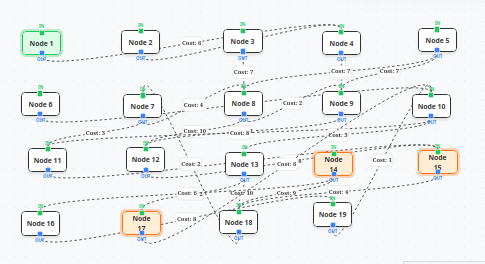
\includegraphics[width=0.9\textwidth]{images/random_graph.png}
    \caption{The main interactive canvas of the visualizer, displaying a randomly generated graph topology with explicit nodes, directional edges, and assigned computational costs.}
    \label{fig:main_canvas}
\end{figure}
\vspace{2cm}

\subsection{Toolkit and Node State Representation}

The environment also features a toolbar (Graph Tools), which dynamically adapts its available actions based on the user's element selection:

\begin{figure}[htbp]
    \centering
    \begin{minipage}{0.45\textwidth}
        \centering
        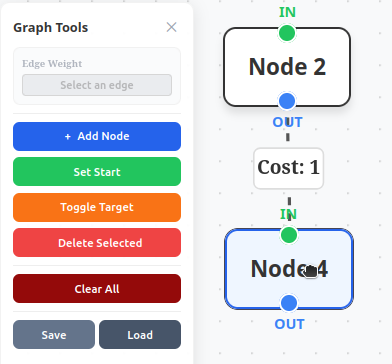
\includegraphics[width=0.8\textwidth]{images/graph_tools_selected_node.png}
        \caption{Toolbar options available when a node is actively selected.}
        \label{fig:tools_node}
    \end{minipage}\hfill
    \begin{minipage}{0.45\textwidth}
        \centering
        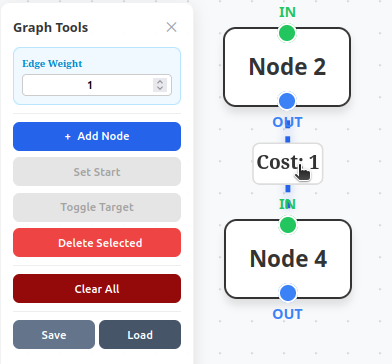
\includegraphics[width=0.8\textwidth]{images/graph_tools_selected_edge.png}
        \caption{Toolbar options available when an edge is actively selected.}
        \label{fig:tools_edge}
    \end{minipage}
\end{figure}

\begin{itemize}
    \item When a \textit{node} is selected the toolbar activates specific controls allowing the user to change the designated role of a node (See Figure \ref{fig:tools_node}). Users can set a unique starting point (\texttt{Set Start}), mark it as one of the multiple targets (\texttt{Toggle Target}), or remove it entirely (\texttt{Delete Selected}). Furthermore, the state of a node can also be alter by the underlying algorithm being run. For example a \textbf{Visited Node} will appear different to a \textbf{Path Node}. This visual distinction is necessary in order to distinguish between nodes that were explored and nodes that were permanently settled (See Figure \ref{fig:node_states}). 
    \begin{figure}[h]
        \centering
        \begin{subfigure}[b]{0.3\linewidth}
            \centering
            
\includegraphics[width=\linewidth]{tex/images/node_simple.png}
            \caption{Neutral State}
            \label{subfig:simple}
        \end{subfigure}
        \hfill
        \begin{subfigure}[b]{0.3\linewidth}
            \centering
            
\includegraphics[width=\linewidth]{tex/images/node_selected.png}
            \caption{Selected State}
            \label{subfig:selected}
        \end{subfigure}
        \hfill
        \begin{subfigure}[b]{0.3\linewidth}
            \centering
            
\includegraphics[width=\linewidth]{tex/images/node_start.png}
            \caption{Start State}
            \label{subfig:start}
        \end{subfigure}
        \begin{subfigure}[b]{0.3\linewidth}
            \centering
            
\includegraphics[width=\linewidth]{tex/images/node_target.png}
            \caption{Target State}
            \label{subfig:target}
        \end{subfigure}
        \hfill
        \begin{subfigure}[b]{0.3\linewidth}
            \centering
            
\includegraphics[width=\linewidth]{tex/images/node_pq.png}
            \caption{Priority Queue State}
            \label{subfig:prio-queue}
        \end{subfigure}
        \hfill
        \begin{subfigure}[b]{0.3\linewidth}
            \centering
            
\includegraphics[width=\linewidth]{tex/images/node_visited.png}
            \caption{Visited State}
            \label{subfig:visited}
        \end{subfigure}
        \begin{subfigure}[b]{0.3\linewidth}
            \centering
            
\includegraphics[width=\linewidth]{tex/images/node_path.png}
            \caption{Path State}
            \label{subfig:path}
        \end{subfigure}
        
        \caption{Visual vocabulary for node states. The color-coded system tracks a node's "status" during execution, distinguishing between unexplored, active priority queue frontiers, settled nodes, and the final optimal path.}
        \label{fig:node_states}
    \end{figure}
    \vspace{5cm}

    \item When an \textit{edge} is selected (See Figure \ref{fig:tools_edge}), the toolbar activates an \texttt{Edge Weight} input space, allowing the user to edit the value of the selected edge's weight. Similar to the nodes, the corresponding color of an edge may change depending on its state while and after running an algorithm (See Figure \ref{fig:edge_legend}).
    \begin{figure}
        \centering
        
\includegraphics[width=0.3\linewidth]{tex/images/edge_legend.png}
        \caption{Visual representation of edge states. Similar to nodes, edges dynamically update their color, highlighting their role during and after execution.}
        \label{fig:edge_legend}
    \end{figure}
\end{itemize}
\vspace{1cm}
\newpage

To further enhance user experience, the visualizer enables the user with global topology management actions (See Figure \ref{fig:graph_actions}). Users can completely clear the canvas by utilizing \texttt{Clear All} function, save or load\footnote{This function is achieved by utilizing the browser's native File API to package the graph state and trigger a local file download} specific user built graphs as a JSON object to local storage using the \texttt{Save}/\texttt{Load} functionality, or instantly generate a \texttt{Random Graph}, or a Pre-Built \texttt{Trap Scenario} (See Section \ref{subsec:trap}) which showcases the advantage of \texttt{DIJKSTRA-PREDICTION}. 


\begin{figure}[htbp]
    \centering
    
\includegraphics[width=0.4\textwidth]{tex/images/graph_tools_graph_actions.png}
    \caption{The global graph management toolkit. These controls allow users to load or save the current topology of any graph in their local files, clear and reset the 2d canvas, or generate a random graph topology or trap scenario (based on internal rules).}
    \label{fig:graph_actions}
\end{figure}

Furthermore, as user generated graphs may grow in scale and complexity, navigating an expanding 2D canvas may become quite challenging. To combat this issue, the visualizer uses a suite of view-port controls. Users can dynamically pan and adjust the zoom level of the workspace\footnote{Can also be controlled with the mouse using the scroll wheel.}, lock the interactivity with the graph or even automatically fit the graph in view (See Figure \ref{fig:view_utils}). User can also utilize a mini-map to have a quick grayscale view of the environment and help traverse it instantly (see Figure \ref{fig:minimap})


\begin{figure}[h]
    \centering
    \begin{subfigure}[b]{0.23\linewidth}
        \centering
        
\includegraphics[height=\linewidth]{tex/images/enviroment_tools.png}
        \caption{View-port}
        \label{subfig:simple}
    \end{subfigure}
    \hfill
    \begin{subfigure}[b]{0.36\linewidth}
        \centering
        
\includegraphics[width=\linewidth]{tex/images/before_fit.jpg}
        \caption{Starting View}
        \label{subfig:selected}
    \end{subfigure}
    \hfill
    \begin{subfigure}[b]{0.36\linewidth}
        \centering
        
\includegraphics[width=\linewidth]{tex/images/after_fit.jpg}
        \caption{After Fit View}
        \label{subfig:start}
    \end{subfigure}
    \caption{Demonstration of the view-port controls. Utilizing the "Fit-to-Screen" functionality allows the user to instantly readjust the canvas from a tightly zoomed-in section (b) to a comprehensive, centered overview of the entire graph topology (c).}
    \label{fig:view_utils}
\end{figure}

\begin{figure}
    \centering
    
\includegraphics[width=0.5\linewidth]{tex/images/minimap.png}
    \caption{The dynamic minimap interface. This component provides an overview of the 2D canvas, ensuring users maintain awareness and control.}
    \label{fig:minimap}
\end{figure}
\vspace{10cm}


\subsection{Trap Scenario}
\label{subsec:trap}

As depicted in Figure \ref{fig:trap_scenario_canvas}, this pre-built scenario consists of a low-cost linear path leading towards the target, which eventually branches out into multiple high-cost dead-ends (traps). This topology is specifically generated by the visualizer to highlight the differences between \texttt{DIJKSTRA} and \texttt{DIJKSTRA-PREDICTION}.

\begin{figure}[htbp]
    \centering
    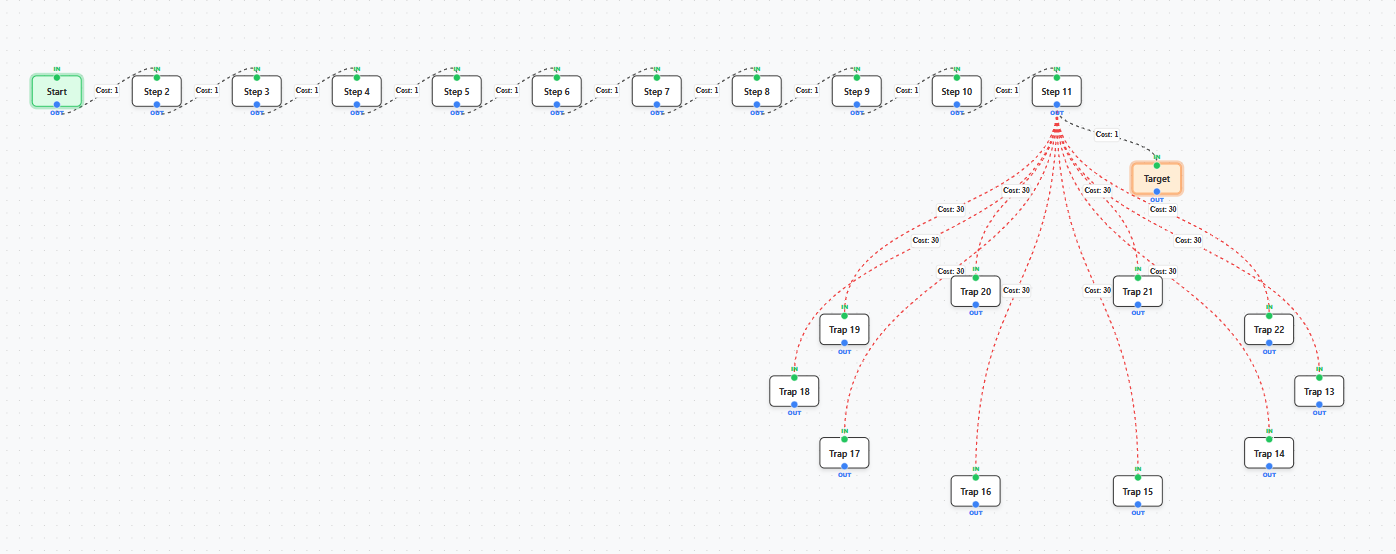
\includegraphics[width=\textwidth]{images/trap_scenario.png}
    \caption{The Pre-Built Trap Scenario topology generated by the visualizer. High-cost trap nodes branch out near the target to highlight the pruning efficiency of the learning-augmented approach.}
    \label{fig:trap_scenario_canvas}
\end{figure}

To demonstrate the difference, users may executes both algorithms on this trap scenario. Figure \ref{fig:trap_comparison} provides a visual comparison of the two algorithms.

When \texttt{DIJKSTRA} reaches the branching node, its exploration mechanism cause all \textit{trap} nodes to be inserted into the priority queue, thus wasting time executing actions.

On the other hand, \texttt{DIJKSTRA-PREDICTION} manages to compute a $P$ threshold value by step $i_0 = 10$ effectively pruning all trap nodes and saving on computational cost.
\newpage

\begin{figure}[htbp]
    \centering
    \begin{subfigure}[b]{0.48\textwidth}
        \centering
        
\includegraphics[width=\linewidth]{tex/images/trap_dijkstra.png}
        \caption{\textsc{DIJKSTRA}: All trap nodes are inserted into the search frontier, causing unnecessary priority queue actions.}
        \label{subfig:trap_dijkstra}
    \end{subfigure}
    \hfill
    \begin{subfigure}[b]{0.48\textwidth}
        \centering
        
\includegraphics[width=\linewidth]{tex/images/trap_dijkstra_pred.png}
        \caption{\textsc{DIJKSTRA-PREDICTION}: Trap nodes are successfully pruned by utilizing a prediction threshold.}
        \label{subfig:trap_pred}
    \end{subfigure}
    \caption{Comparative execution of the Trap Scenario. }
    \label{fig:trap_comparison}
\end{figure}


\subsection{In-App Documentation and Notes}
\label{subsec:info}

For the purposes of transparency the application provides documentation and notes via a "Info" button located within the view-port controls toolkit (Figure \ref{subfig:info_button}).

Activating this toggle overlays a panel directly onto the workspace (Figure \ref{subfig:info_panel}). The panel contains info, setups, as well as findings, all together with a direct link to this thesis paper to help guide users.

\begin{figure}[htbp]
    \centering
    \begin{subfigure}[b]{0.15\textwidth}
        \centering
        
\includegraphics[width=\linewidth]{tex/images/info_button.png}
        \caption{Info Button}
        \label{subfig:info_button}
    \end{subfigure}
    \hfill
    \begin{subfigure}[b]{0.75\textwidth}
        \centering
        
\includegraphics[width=\linewidth]{tex/images/info_panel.jpg}
        \caption{Thesis Notes Panel}
        \label{subfig:info_panel}
    \end{subfigure}
    \caption{The in-app documentation utility. The contextual Info button (a) activates the Thesis Notes modal (b), providing a unified interface for logging experimental observations and theoretical parameters.}
    \label{fig:info_feature}
\end{figure}


\subsection{Algorithm Selection}
\label{subsec:algorithm_selection}
The user has the ability to select which algorithm to execute. This is enabled through a drop-down selection interface on the toolbar (Graph Tools), See Figure \ref{fig:run_algorithms}.

\begin{figure}[htbp]
    \centering
    \begin{subfigure}[b]{0.45\textwidth}
        \centering
        
\includegraphics[width=0.7\linewidth]{tex/images/dropdown_closed.png}
        \caption{Expanded Drop-down Menu}
        \label{subfig:menu_expanded}
    \end{subfigure}
    \hfill
    \begin{subfigure}[b]{0.45\textwidth}
        \centering
        
\includegraphics[width=0.7\linewidth]{tex/images/dropdown_open.png}
        \caption{Active Selection and Execution}
        \label{subfig:menu_execution}
    \end{subfigure}
    \caption{The algorithm selection interface. Users can expand the menu to choose between models (a). Once selected, the execution button triggers the backend processing (b).}
    \label{fig:run_algorithms}
\end{figure}

Upon clicking \texttt{Run}, the front-end process prepares the graph. It packages the topology into a structured JSON payload. This payload is then transmitted to the back-end to be processed. 


\subsection{The Playback Engine and State Management}
\label{subsec:playback_engine}

When the back-end returns the execution history (\texttt{visited\_steps} and \newline \texttt{queue\_steps}), a \texttt{buildTimeline} function executes. 

The animation is driven by (\texttt{currentStep}) and a timer. As the timer passes, the \texttt{applyStep} function modifies the CSS classes of the React Flow elements, visually distinguishing the priority queue without modifying the graph data structure.

To showcase the process, Figure \ref{fig:playback_sequence} demonstrates a step-by-step execution of the classic \textsc{DIJKSTRA} algorithm. Nodes and edges swap through node states (See Figures \ref{fig:node_states} and \ref{fig:edge_legend}) based on the back-end. Initially, neighbors of the active node are inserted into the \textit{priority queue}. In the  frames, nodes are extracted from the \textit{priority queue} and marked as permanently visited. Upon reaching the target, the engine solves the \texttt{paths} array from the payload, highlights the final optimal route.

\begin{figure}[h]
    \centering
    \begin{subfigure}[b]{0.35\textwidth}
        \centering
        
\includegraphics[width=\linewidth]{tex/images/run_step_1.png}
        \caption{Starting state of the graph. All nodes remain unexplored.}
        \label{subfig:step1}
    \end{subfigure}
    \hfill
    \begin{subfigure}[b]{0.35\textwidth}
        \centering
        
\includegraphics[width=\linewidth]{tex/images/run_step_2.png}
        \caption{Neighbors of the start node are inserted into the priority queue.}
        \label{subfig:step2}
    \end{subfigure}
    
    \begin{subfigure}[b]{0.35\textwidth}
        \centering
        
\includegraphics[width=\linewidth]{tex/images/run_step_3.png}
        \caption{ A node is extracted from the queue (visited).}
        \label{subfig:step3}
    \end{subfigure}
    \hfill
    \begin{subfigure}[b]{0.35\textwidth}
        \centering
        
\includegraphics[width=\linewidth]{tex/images/run_step_4.png}
        \caption{The algorithm continues exploring nodes in the queue.}
        \label{subfig:step4}
    \end{subfigure}
    \caption{Sequential playback of the classic \textsc{DIJKSTRA} algorithm. The playback engine updates the visual state of nodes and edges at each time step.}
    \label{fig:playback_sequence}
\end{figure}

The logic of the playback engine relies on two primary procedures (Algorithms \ref{alg:build_timeline} and \ref{alg:apply_step}). The \textsc{BUILD-TIMELINE} algorithm processes the raw execution trace. By checking the state of the priority queue at each step, it filters out redundant operations (e.g. No changes in priority queue) and constructs a sequence of animation frames, without duplicates. 

The \textsc{APPLY-STEP} algorithm take care of the visual rendering. Given a specific frame from the timeline, it resets the canvas and applies the correct CSS classes based on the previously states Node and Edge States (See Figures \ref{fig:node_states} and \ref{fig:edge_legend}). The algorithm transitions nodes between the \textit{priority queue} state and the \textit{visited} state. When the timeline reaches the final "path" frame, it highlights the final optimized shortest path.
\vspace{0.5cm}

\begin{algorithm}[H]
\caption{BUILD-TIMELINE(data)} \label{alg:build_timeline}
$timeline = []$\;
$lastQueueKey = null$\;

\ForEach{$step$ \textnormal{in} $data.visited\_steps$}{
    $i = \textnormal{index of } step$\;
    $queueSnapshot = \textnormal{GET-SNAPSHOT}\footnote{Explanation on State Snapshots on Section \ref{subsec:state_snapshots}}(data.queue\_steps, i)$\;
    $queueKey = \textnormal{HASH}(queueSnapshot)$ \tcp*{generate unique state key}
    
    \If{$queueKey \neq lastQueueKey$}{\tcp{only add to timeline if there's a change}
        $timeline\textnormal{.APPEND}(\{type: \text{"queue"}, index: i\})$ \tcp*{record queue update}
        $lastQueueKey = queueKey$\;
    }
    $timeline\textnormal{.APPEND}(\{type: \text{"visit"}, index: i+1\})$ \tcp*{record node visit}
}

$timeline\textnormal{.APPEND}(\{type: \text{"path"}\})$ \tcp*{final resolution step}
\Return $timeline$\;
\end{algorithm}

\begin{algorithm}[H]
\caption{APPLY-STEP(timelineIndex, data, timeline)} \label{alg:apply_step}
RESET-VISUAL-STATES() \tcp*{clear all visual node/edge classes}
$step = timeline[timelineIndex]$\;

\eIf{$step.type == \text{"path"}$}{
    HIGHLIGHT-ALL($data.visited\_steps$, "visited")\;
    HIGHLIGHT-PATH($data.paths$, "path-node") \tcp*{highlight optimal route}
    UPDATE-UI-STATS($data.queue\_steps[-1]$) \tcp*{display final P and B}
}{
    $i = step.index$\;
    $visitedSet = \textnormal{GET-VISITED-UNTIL}(data.visited\_steps, i)$\;
    $queueSet = \textnormal{GET-QUEUE-SNAPSHOT}(data.queue\_steps, i)$\;

    \If{$step.type == \text{"visit"}$}{
        $queueSet\textnormal{.REMOVE}(data.visited\_steps[i])$ \tcp*{node transitions to visited}
    }

    HIGHLIGHT-NODES($visitedSet$, "visited")\;
    HIGHLIGHT-NODES($queueSet$, "queue-node")\;
    UPDATE-UI-STATS($data.queue\_steps[i]$) \tcp*{update real-time P and B}
}
\end{algorithm}
\vspace{0.5cm}


\subsection{Animation Controls}
\label{subsec:navigation_animation}
To give users full control over the playback engine rather than automatically and instantaneously rendering the final shortest path, the environment by default is designed to automatically execute the \texttt{applyStep} updates with a timed delay (\textit{1000ms/1s}), and even further provides the user with an interactive bottom toolkit for \texttt{Pause} and \texttt{Play} functionality, as well as \texttt{Next Step} and \texttt{Previous Step} options (See Figure \ref{fig:animation_tools}).

\begin{figure}[htbp]
    \centering
    
\includegraphics[width=0.5\linewidth]{tex/images/animation_tools.png}
    \caption{Interactive animation playback controls. This toolkit enables, frame-by-frame traversal of the algorithm's execution history.}
    \label{fig:animation_tools}
\end{figure}

\section{Backend Architecture and API Design}
\label{sec:backend}

The back-end of the visualizer is developed using Python and specifically \texttt{FastAPI}. This framework was selected for its performance and support for REST (Representational State Transfer) APIs. To allow secure, cross-domain communication, we utilise Cross-Origin Resource Sharing (CORS), preventing cross-site suspicious request.

\subsection{Data Validation and Payload Structure}
\label{subsec:data_validation}

We ensure that the graph created by the user in the React front-end environment is correctly processed through data validation. We achieve this by utilizing \texttt{Pydantic} models. 

\begin{itemize}
	\item The system defines an \texttt{EdgeModel} class to correctly store all useful information about an edge (\texttt{source}, \texttt{target}, and \texttt{weight}). 
	\item The \texttt{GraphPayload} defines the JSON structure of the incoming request, containing the \texttt{startNode}, a list of \texttt{targetNodes}, and the complete arrays of nodes and edges.
\end{itemize}

\subsection{The Endpoint Communication}
\label{subsec:solver_endpoint}

The communication between the front-end and back-end occurs through a single \texttt{POST} endpoint denoted as \texttt{/solve}. Upon receiving a request, the back-end parses the JSON payload into the \texttt{GraphPayload} model we saw before. 

The Endpoint then precedes to execute the algorithms \texttt{DIJKSTRA} and \texttt{DIJKSTRA-PREDICTION}, one after the other, on the same graph data. After executing the endpoint bundles the result (i.e. the \texttt{visited\-steps} and \texttt{queue\-steps} arrays). After this response reaches the front-end it can be processed by the playback engine to deliver the animation to the user depending on the algorithm chosen (See Section \ref{subsec:algorithm_selection})

\subsection{Algorithmic Translation and State Snapshots}
\label{subsec:state_snapshots}
The algorithms, \texttt{DIJKSTRA} and \texttt{DIJKSTRA-PREDICTION}, were both modified for the purpose of visualizing the results. A standard implementation would simply return the final optimal path found by the two algorithms, but for our goal we require a visualization of a \textit{snapshot} of the state of the nodes at every step of the algorithmic execution. 

Basically, as we stated before, our goal is to showcase the difference in the number of priority queue operations, which lead \texttt{DIJKSTRA-PREDICTION} to a faster running time. To achieve this, we utilize the Python \texttt{heapq} library, in order to mantain the priority queue data structure efficiently. At every step, the algorithms saves the exact state of the queue. For \texttt{DIJKSTRA-PREDICTION}, the algorithm also save the pruning bound ($B$).

\subsection{Oracle Integration and Data Structures}
\label{subsec:oracle_integration}

A big challenge when dealing with any algorithm with predictions is the integration of the machine learning oracle into the execution loop. The algorithm, \texttt{DIJKSTRA-PREDICTION} achieves this without an expensive computational cost through the use of the \texttt{joblib} library which loads the pre-trained model (Multi-Layer Perceptron - MLP) into the server's memory.

During the initial $i_0$ iterations of the algorithm, the back-end creates the trace by appending the lower bound $d_i$ together with the upper bound $B_i$ (See Section \ref{sec:dijkstra-prediction}) of each step. Once the trace is complete, it is formatted into a \texttt{NumPy} array and passed to the oracle to make a prediction $P$, for it to be used as a threshold. 

Lastly, the Reserve Set ($R$) was implemented using a Python hash map (dictionary), thus ensuring $O(1)$ execution time when executing any insertions, lookup and deletion. This allows the \texttt{UPDATE-PREDICTION} routine to be able to very quickly extract nodes from the Reserve Set ($R$) and re-insert them into the priority queue.

\subsection{Performance Tracking and Metrics Collection}
\label{subsec:performace_tracking}

Moving away from the visualization the backend collects data and metrics on the performance of the algorithms.

Because \textsc{DIJKSTRA-PREDICTION} maintains the  same complexity bound of $\mathcal{O}(m+n\log n)$ as classic \textsc{DIJKSTRA}, theoretical and visual analysis alone is not enough to evaluate its performance. Therefore, we utilize these metrics to accurately quantify the actual computational cost saved.

An optional \texttt{collect\_stats} parameter is integrated into the algorithm. When activated, it allows for tracking of every action with the data structures:


\begin{itemize}
    \item \textbf{Priority Queue Operations:} The algorithms record the number of insertions (\texttt{pq\_pushes}) and extractions (\texttt{pq\_pops}). They also track duplicate encounters (\texttt{pq\_skips}), which occur when a shorter path to an already enqueued node is discovered, bypassing unnecessary heap evaluations.
    \item \textbf{Reserve Set Operations:} Specific to \textsc{DIJKSTRA-PREDICTION}, the system logs the number of nodes pruned and stored in the fallback dictionary (\texttt{r\_inserts}), as well as the nodes recovered during an \texttt{UPDATE-PREDICTION} routine (\texttt{r\_rescues}).
\end{itemize}

Through this metrics, the algorithm allows us to move away from the theoretical background and claims in Chapter \ref{ch:learning_augmented}, and compare the results between \texttt{DIJKSTRA-PREDICTION}, \texttt{DIJKSTRA}, and other traditional Machine Learning approaches in Chapter \ref{ch:experimentation}.

\subsection{Full Overview of a Sequence Flow}
\label{subsec:sequence_flow}

To aid in the understanding of the synchronization between the front-end visual user interface and the back-end computational executions, we define the complete UML sequence diagram in Figure \ref{fig:uml_diagram}. 

\begin{figure}[h]
    \centering
    
\includegraphics[width=1\linewidth]{tex/images/uml.drawio.png}
    \caption{UML Sequence Diagram illustrating the synchronous client-server execution loop. The front-end serializes the current canvas topology, which is then sequentially processed by both routing algorithms to extract performance metrics and step-by-step state animations.}
    \label{fig:uml_diagram}
\end{figure}

The diagram details the life cycle of a routing request. The operations pass through four different discrete phases:

\begin{enumerate}
    \item \textbf{React Front-End:} The process starts when the user presses on the execution button. The front-end packages the active nodes, directed edges, explicit weights, and multiple target states into a  structure following the \texttt{GraphPayload} Pydantic schema. This object is transmitted across domains via an HTTP \texttt{POST} request.
    \item \textbf{FastAPI Server:} Upon receipt, the \texttt{FastAPI} middleware performs schema validation. Only after passing validation does the server sequentially pass the computation to the algorithms.
    \item \textbf{Python Solvers:} The modules execute both classic \textsc{DIJKSTRA} and \textsc{DIJKSTRA-PREDICTION}. During execution, the internal states are recorded at every step, logging priority queue actions, reserve set operations, and specific bounding parameters ($B$ and $P$). Once finished, the execution data and performance metrics are packaged into a unified response payload.
    \item \textbf{Animation Playback:} The bundled JSON payload is returned to the client via an HTTP 200 OK response. The front-end playback engine receives this data, executes the \texttt{buildTimeline()} procedure to prune redundant frames where no changes occured, and begins the cyclic execution of \texttt{applyStep()} to update the visual states of the elements of the graph.
\end{enumerate}
 
% \chapter{Experimentation}
\label{ch:experimentation}
The theoretical analysis on Chapter \ref{ch:learning_augmented} provides the mathematical guarantees, but as previously stated, $Big$ $O$ Notation fails to capture the algorithms true efficiency gained from the machine learning aspect of \texttt{DIJKSTRA-PREDICTION}

This chapter therefore, presents a comprehensive experimental analysis and review of \texttt{DIJKSTRA-PREDICTION}, bench-marked against the classical \texttt{DIJKSTRA} algorithm, focusing entirely on the true reduction to the priority queue operations, resulting in an overall reduction in execution time.

More specifically, our experimental setup aims to evaluate:
\begin{itemize}
    \item The direct trade-off between the machine learning technique and the classical approach.
    \item The behavior of the Reserve Set ($R$) and thhe frequency on which the \texttt{UPDATE-PREDICTION} routine executes.
    \item The performance gain/loss between different oracle architectures, such as different neural (Multi-Layer Perceptrons) and gradient boosting models (XGBoost).
\end{itemize}

Our experiments are performed across tens of thousands of randomly generated graphs to ensure our evaluations are unbiased.
\newpage

\section{Dataset and Trace Extraction}
\label{sec:dataset}
Real-life networks, such as city road networks, are often inherently biased, for example with grid-like structures. To combat this issue, inorder to properly train and evaluate our machine learning oracle, we utilized the Erdős-Rényi\cite{erdos1960evolution} $G(n, p)$ random graph model to construct unbiased experimental scenarios, similar to Feijen and Schäfer\cite{feijenDijkstrasAlgorithmPredictions2023}. 


\subsection{Random Graph Generation (Erdős-Rényi)}
\label{subsec:erdos_renyi}

A custom Python data pipeline (\texttt{generate\_random\_graphs.py}) was developed to construct thousands of random topologies. Each generated graph $G=(V,E)$ is build according to the following rules:
\begin{itemize}
    \item \textbf{Vertices ($n$):} Each graph consists of precisely $n = 1000$ nodes.
    \item \textbf{Edge Probability ($p$):} To simulate realistic network sparsity, the expected out-degree of each node was set to $c = 8$. The probability of a directed edge existing between any two nodes is defined as $p = c / n = 0.008$.
    \item \textbf{Edge Weights ($w$):} To guarantee compliance with \textsc{DIJKSTRA}'s non-negative constraint, the weight $w(u,v)$ of every generated edge is drawn from a uniform random distribution between $(0, 1)$.
    \item \textbf{Target Nodes ($T$):} The expected number of target nodes per graph was set to $f = 20$. Each node is independently assigned as a target with probability $q = f / n = 0.02$. A fallback mechanism ensures that at least one valid target exists in $T$ if the pipeline results in an empty set.
\end{itemize}

The logic for generating these graphs is given in Algorithm \ref{alg:erdos}.

\begin{algorithm}[H]
\label{alg:erdos}
\caption{ERDOS-RENYI-GENERATOR ($n, c, f$)}
$p = c / n$, $q = f / n$\;
$V = \{0, 1, \dots, n-1\}$\;
$s = \text{RANDOM-INTEGER}(0, n-1)$\;
$T = \emptyset$, $E = \emptyset$\;

\tcp{Target Node Selection}
\For{$v \in V \setminus \{s\}$}{
    \If{$\text{RANDOM}() < q$}{
        $T \leftarrow T \cup \{v\}$\;
    }
}
\If{$T == \emptyset$}{
    $T \leftarrow \{\text{RANDOM-INTEGER}(0, n-1) \neq s\}$ \tcp*{Fallback}
}

\tcp{Edge Generation}
\For{$u \in V$}{
    $out\_degree \sim \mathcal{B}(n-1, p)$ \tcp*{Sample from binomial distribution}
    \If{$out\_degree > 0$}{
        $targets \leftarrow \text{RANDOM-SAMPLE}(V \setminus \{u\}, out\_degree)$\;
        \For{$v \in targets$}{
            $w \sim (0, 1)$ \tcp*{Sample from uniform distribution}
            $E \leftarrow E \cup \{(u, v, w)\}$\;
        }
    }
}
\Return $G=(V, E), s, T$
\end{algorithm}
\newpage

\subsection{Trace Extraction}
\label{subsec:trace_extraction}
In order to train our machine learning networks we require a supervised learning dataset. To achieve this each graph in our dataset must be converted into a feature vector $X$ (the algorithmic $trace$)\footnote{Explanation for the structure of the $trace$ was given in Section \ref{sec:prinicples}} and a corresponding label $y$ (the true shortest path).

For every generated graph, a \texttt{DIJKSTRA} execution is initiated from a randomly selected source node $s$. The algorithm executes exactly $i_0 = 10$ steps. At each step $i \in \{1, 2, \dots, i_0\}$, the system records two values:

\begin{enumerate}
    \item $d_i$: The distance of the node currently extracted from the priority queue (representing the expanding lower bound).
    \item $B_i$: The current best-known upper bound to any target $t \in T$. If no target has been discovered yet, this is represented as $0.0$ for the model (to avoid \texttt{Infinity} errors).
\end{enumerate}


When this process finalizes, it returns a 20-dimensional feature vector array $X = [d_1, B_1, d_2, B_2, \dots, d_{10}, B_{10}]$. After the initial $i_0$ steps, the algorithm resumes execution until it settles the first target node, recording the true shortest path distance $D$. This value is the target label $y$ for our supervised learning models.

If the algorithm happens to find target $t \in T$ in the first $i_0$ steps, then the graph is discarded from the training set, as it contains less than the required 20 features.

Through this pipeline, we generated a total of 80,000 valid graphs for the training of the models. For each graph, their corresponding $trace$ was then compiled into a final unified CSV dataset, ready to be used. 

The execution mechanics for extracting the supervised feature vector $X$ and the label $y$ from any given graph are detailed in Algorithm \ref{alg:trace_extract}.


\begin{algorithm}[htbp]
\caption{TRACE-EXTRACTOR ($G, s, T, i_0$)}
\label{alg:trace_extract}
$d(v) = \infty$ \textbf{for all} $v \in V$, $d(s) = 0$\;
PQ.INSERT$(s, 0)$\;
$B = \infty$, $X = \emptyset$, $y = \text{NULL}$\;
$i = 0$, $S = \emptyset$ \tcp*{Settled nodes}

\While{\textbf{not} PQ.EMPTY()}{
    $u = \text{PQ.REMOVE-MIN}()$\;
    \If{$u \in S$}{\textbf{continue}}
    
    $S \leftarrow S \cup \{u\}$\;
    $i = i + 1$\;
    
    \If{$i \le i_0$}{
        \eIf{$B == \infty$}{
            $B_{formatted} = 0.0$\;
        }{
            $B_{formatted} = B$\;
        }
        $X \leftarrow X \cup \{d(u), B_{formatted}\}$ \tcp*{Append to feature vector}
    }
    
    \If{$u \in T$}{
        $y = d(u)$ \tcp*{Optimal shortest path found}
        \textbf{break}\;
    }
    
    \For{$(u,v) \in E$}{
        \If{$v \in S$}{\textbf{continue}}
        $tent = d(u) + w(u,v)$\;
        \If{$v \in T$}{
            $B = \min(B, tent)$\;
        }
        \If{$tent < d(v)$}{
            $d(v) = tent$\;
            PQ.INSERT$(v, tent)$\;
        }
    }
}

\If{$y == \text{NULL}$ \textbf{or} $i \le i_0$}{
    \Return \text{INVALID} \tcp*{Graph is invalid for training}
}
\Return $X, y$
\end{algorithm}

\section{Oracle Architecture and Model Training}
\label{sec:oracle_training}

With the generation of the 80,000 algorithmic traces and their optimal shortest path distances, the problem is structured as a supervised regression task. The objective is to train a machine learning oracle capable of accurately mapping the $i_0$-step algorithmic trace $X$ to the predicted target distance $P$. 

The dataset was split into a training set (80\%) and a testing set (20\%), for evaluation purposes before the final benchmark test. To guarantee proper experimental tracking, all hyperparameter configurations and resulting metrics were tracked utilizing the \texttt{MLflow} platform.  

We evaluate two machine learning models for the role of the prediction oracle: Multi-Layer Perceptrons (MLP)\cite{rumelhartLearningRepresentationsBackpropagating1986} and Gradient Boosting Decision Trees (XGBoost)\cite{chenXGBoostScalableTree2016}.


\subsection{Multi-Layer Perceptron (MLP) Configurations}
\label{subsec:mlp_training}

Similar to Feijen and Schäfer we utilized the \texttt{MLPRegressor}. The models were configured to train for a maximum of 1000 iterations (\texttt{max\_iter}). 

We tested five different hidden-layer architectures, utilizing two hidden layers of varying widths: $(8, 8)$, $(16, 16)$, $(32, 32)$, $(64, 64)$, and $(128, 128)$.

\begin{figure}[htbp]
    \centering
    
\includegraphics[width=0.8\linewidth]{tex/images/mlp_mae.png}
    \caption{Mean Absolute Error (MAE) evaluation of various MLP architectures}
    \label{fig:mlp_mae}
    
    \vspace{0.5cm} % Προσθέτει λίγο κενό ανάμεσα στις δύο εικόνες
    
    
\includegraphics[width=0.8\linewidth]{tex/images/mlp_mape.png}
    \caption{Mean Absolute Percentage Error (MAPE) evaluation of various MLP architectures}
    \label{fig:mlp_mape}
\end{figure}
\newpage


\begin{table}[h]
\centering
\caption{Performance metrics of various MLP architectures.}
\label{tab:mlp_metrics}
\renewcommand{\tabularxcolumn}[1]{m{#1}}
\begin{tabularx}{\textwidth}{
    >{\centering\arraybackslash}X 
    >{\centering\arraybackslash}X 
    >{\centering\arraybackslash}X
}
\toprule
\textbf{Model Architecture} & \textbf{Mean Absolute Error (MAE)} & \textbf{Mean Absolute Percentage Error (MAPE)} \\ \midrule
128x128 & 0.0641008 & 0.12911040 \\
64x64   & 0.0644093 & 0.12737545 \\
32x32   & 0.0647925 & 0.12926555 \\
16x16   & 0.0668187 & 0.13688045 \\
8x8     & 0.0706973 & 0.14335474 \\ \bottomrule
\end{tabularx}
\end{table}


According to the training results (see Figures \ref{fig:mlp_mae} and \ref{fig:mlp_mape} and Table \ref{tab:mlp_metrics}), scaling the model's architecture provides an improvement, especially in the beginning. The $(8, 8)$ architecture results in a \(\approx \)0.0706 MAE value and a \(\approx \)0.1433 MAPE value. The $(16, 16)$ architecture shows a notable improvement with a \(\approx \)0.0668 MAE value and a \(\approx \)0.1368 MAPE value. Further scaling the model to a $(32, 32)$ architecture shows a drop into a  \(\approx \)0.0647 MAE value and a  \(\approx \)0.1292 MAPE value, but notably, continuing to scale the architecture into $(64, 64)$, and $(128, 128)$ yields no measurable improvement in either metric, introducing the law of diminishing returns.

Since the oracle model executes synchronously within the loop of the \texttt{DIJKSTRA-PREDICTION} algorithm, we require our model to be lightweight, so as to not incur heavy computational loads leading to an overall worse performance in time execution compared to \texttt{DIJKSTRA}. Notably for our interactive environment, we deployed an MLP architecture of $(16, 16)$ following Feijen's and Schäfer's chosen oracle.

\subsection{Gradient Boosting (XGBoost) Variants}
\label{subsec:xgboost_training}

While Feijen and Schäfer deployed an MLP to act as an oracle, for our experiments we consider the alternative use of a tree ensemble method. XGBoost often achieves superior performance and faster inference time on tabular data.

We trained three XGBoost architectures. For the purposes of this thesis we denote an XGBoost configuration as $\text{XGBoost}(n, d, \eta)$ where $n$ is the number of estimators, $d$ is the maximum depth, and $\eta$ is the learning rate:

\begin{itemize}
    \item \textbf{XGBoost Fast (100, 3, 0.1):} Configured with 100 estimators, a maximum tree depth of 3, and a learning rate of 0.1. This variant is designed for fast inference, minimizing the time reduction taken for the prediction of the value P.
    \item \textbf{XGBoost Medium (200, 4, 0.05):} Configured with 200 estimators, a maximum tree depth of 4, and a learning rate of 0.05. This variant was designed as a middle ground.
    \item \textbf{XGBoost Deep (300, 5, 0.05):} Configured with 300 estimators, a maximum tree depth of 5, and a learning rate of 0.05. This variant is designed to minimize the error of the prediction.
\end{itemize}

\begin{table}[h]
\centering
\caption{Performance metrics of the evaluated XGBoost architectures.}
\label{tab:xgboost_metrics}
\renewcommand{\tabularxcolumn}[1]{m{#1}}
\begin{tabularx}{\textwidth}{
    >{\centering\arraybackslash}X 
    >{\centering\arraybackslash}X 
    >{\centering\arraybackslash}X
}
\toprule
\textbf{Model Architecture} & \textbf{Mean Absolute Error (MAE)} & \textbf{Mean Absolute Percentage Error (MAPE)} \\ \midrule
XGBoost Deep (300,5,0.05)  & 0.0637316 & 0.1271240 \\
XGBoost Medium (200,4,0.05) & 0.0651171 & 0.1303728 \\
XGBoost Fast (100,3,0.1)  & 0.0669162 & 0.1345042 \\ \bottomrule
\end{tabularx}
\end{table}


\begin{figure}[htbp]
    \centering
    
\includegraphics[width=0.8\linewidth]{tex/images/xgboost_mae.png}
    \caption{Mean Absolute Error (MAE) evaluation of XGBoost variants}
    \label{fig:xgboost_mae}
    
    \vspace{0.5cm} 
    
    
\includegraphics[width=0.8\linewidth]{tex/images/xgboost_mape.png}
    \caption{Mean Absolute Percentage Error (MAPE) evaluation of XGBoost variants.}
    \label{fig:xgboost_mape}
\end{figure}
\newpage

According to the training results (See Figure \ref{fig:xgboost_mae} and \ref{fig:xgboost_mape}, and Table \ref{tab:xgboost_metrics}) the gradient boosting approach demonstrates a similar performance to the MLP approach. XGBoost Fast (100,3,0.1) achieved a \(\approx \)0.0669 MAE value and a \(\approx \)0.1345 MAPE value. XGBoost Medium (200,4,0.05) performed slightly better with a \(\approx \)0.0651 MAE value and a \(\approx \)0.1303 MAPE value. Finally, XGBoost Deep (300,5,0.05) performed overall better, with a \(\approx \)0.0637 MAE value and a \(\approx \)0.1271 MAPE value.
Similarly to the MLP deployment, we require the XGBoost model used to be lightweight. 

Despite the performance of the XGBoost models there is a fundamental flaw making them unviable for predictions outside the Erdős-Rényi graph generation model. Decision tree models are notoriously \textit{bad} at extrapolation. In other words, because decision trees partition the feature space into regions and as a result they cannot predict values larger than the maximum target observed during the training phase. For example an XGBoost model trained on the Erdős-Rényi graph generation model ((0,1) weight distribution) would be unable to predict a correct value in our interactive enviroment if a user chose to assign weight weight ranging from 10 to 1000, since the final target value (the final total path distance) is likely to be several times larger than one encountered during training. 

In contrast, MLPs map inputs through mathematical weight transformations, allowing them to extrapolate values to unseen numerical ranges. Therefore, while XGBoost provides sufficient results in our local experiments, the MLP architecture chosen by Feijen and Schäfer remains the best option for a user-driven application.

Still, if trained on a dataset where the training maximum target values remain consistent and relevant in relation to a deployment environment, the extrapolation flaw becomes irrelevant, Therefore, we will still consider the gradient boosting approach in our following experiments. This enables us to evaluate the impact this approach can have on Priority Queue operations and finally overall execution time.
\newpage

\subsection{Evaluating Alternative Architectures}
\label{subsec:alternative_architectures}

Besides Multi-Layer Perceptrons and Gradient Boosting, one can consider using a state-of-the-art model such as Graph Neural Networks (GNNs)\cite{scarselliTheGraphNeuralNetworkModel2009} or Attention-based Transformers\cite{vaswaniAttentionAllYou2023}. These models are better suited for capturing graph topologies and long-range relationships and can predict a $P$ value with higher accuracy thus further reducing the priority queue operations in large scale graphs.

The issue with implementing such models arises when solving for the shortest overall execution time. The computational cost and memory required for their inference phase would be considerably larger compared to more lightweight methods such as MLP and XGBoost. This delay would result in a larger delay for the prediction of the oracle and would therefore render the \texttt{DIJKSTRA-PREDICTION} algorithm slower compared to \texttt{DIJKSTRA}. Consequently, we won't consider heavier models in our experiments.

\section{Comparative Results}
\label{sec:results}

The MAE and MAPE values evaluated in Section \ref{sec:oracle_training} provide insights into the model's accuracy. In order to compare \texttt{DIJKSTRA-PREDICTION} to \texttt{DIJKSTRA} we bench-marked the execution of the two algorithms against each other, utilizing the oracles presented. 

The test set consist of 10,000 generated graph, following the Erdős-Rényi graph generation model (See Section \ref{subsec:erdos_renyi}) with parameters ($n=1000, c=8, f=20$). \texttt{DIJKSTRA-PREDICTION} was set to make a prediction at $i_0 = 10$, and we defined $\alpha = 1.1$ and $\beta = 1.2$.

All resulting data were tracked utilizing the \texttt{MLflow} platform and were exported and visualized using the \texttt{Matplotlib} and \texttt{Seaborn} frameworks. 
\newpage

\subsection{Algorithmic Execution of MLP Oracle Architectures}
\label{subsec:mlp_benchmark}

We begin our evaluation by comparing for the MLP oracle model variants.

Table \ref{tab:mlp_prio} and Figures \ref{fig:mlp_prio} and \ref{fig:mlp_skipped_prio} showcase the average priority queue operations compared to \texttt{DIJKSTRA} and furthermore a comparison on average priority queue operations skipped by each oracle model.

\begin{table}[h]
\centering
\caption{Priority Queue Operations with MLP oracle architectures.}
\label{tab:mlp_prio}
\renewcommand{\tabularxcolumn}[1]{m{#1}}
\begin{tabularx}{\textwidth}{
    >{\centering\arraybackslash}X 
    >{\centering\arraybackslash}X 
    >{\centering\arraybackslash}X
}
\toprule
\textbf{Oracle Model Architecture} & \textbf{Average Priority Queue Operations} & \textbf{Average Priority Queue Operation Skips} \\ \midrule
MLP(128x128) & 139.18 & 243.50 \\
MLP(64x64)   & 138.74 & 243.95 \\
MLP(32x32)   & 138.71 & 243.98 \\
MLP(16x16)   & 139.44 & 243.25 \\
MLP(8x8)     & 138.87 & 243.82 \\ \midrule
\texttt{DIJKSTRA} & 382.7 & -  \\ \bottomrule
\end{tabularx}
\end{table}

\begin{figure}[h]
    \centering
    
\includegraphics[width=1\linewidth]{tex/images/mlp_ops_comparison.png}
    \caption{Average operations achieved via prediction pruning (MLP).}
    \label{fig:mlp_prio}
\end{figure}

\begin{figure}[h]
    \centering
    
\includegraphics[width=1\linewidth]{tex/images/mlp_skipped_ops_comparison.png}
    \caption{Average skipped operations achieved via prediction pruning (MLP).}
    \label{fig:mlp_skipped_prio}
\end{figure}


The classic \texttt{DIJKSTRA} algorithm required an average of 382.7 operations per graph compared to \texttt{DIJKSTRA-PREDICTION} which showcased a significant reduction of more than 60\% leading to an average of $\approx 139$ operations per graph, skipping $\approx 243.5$ operations depending on the oracle model used.

It is important to note that scaling the neural network architecture provided no algorithmic benefit.

We also tracked the behavior of the Reserve Set ($R$). Table \ref{tab:mlp_reserve} and Figures \ref{fig:mlp_r_inserts} and \ref{fig:mlp_r_rescues} showcase the use of the Reserve Set ($R$), both in average reserve set inserts and average reserve set rescues, in order to evaluate its use through out the algorithm.

\begin{table}[h]
\centering
\caption{Reserve Set Operations with MLP oracle architectures.}
\label{tab:mlp_reserve}
\renewcommand{\tabularxcolumn}[1]{m{#1}}
\begin{tabularx}{\textwidth}{
    >{\centering\arraybackslash}X 
    >{\centering\arraybackslash}X 
    >{\centering\arraybackslash}X
}
\toprule
\textbf{Oracle Model Architecture} & \textbf{Average Reserve Set Inserts} & \textbf{Average Reserve Set Rescues} \\ \midrule
MLP(128x128) & 31.36 & 5.92 \\
MLP(64x64)   & 32.52 & 6.64 \\
MLP(32x32)   & 32.63 & 6.73 \\
MLP(16x16)   & 30.99 & 5.80 \\
MLP(8x8)     & 32.57 & 6.83 \\ \bottomrule
\end{tabularx}
\end{table}

\begin{figure}[htbp]
    \centering
    
\includegraphics[width=1\linewidth]{tex/images/mlp_r_inserts_comparison.png}
    \caption{Average node insertions into the Reserve Set (MLP).}
    \label{fig:mlp_r_inserts}
\end{figure}

\begin{figure}[htbp]
    \centering
    
\includegraphics[width=1\linewidth]{tex/images/mlp_r_rescues_comparison.png}
    \caption{Average node rescues triggered during execution (MLP).}
    \label{fig:mlp_r_rescues}
\end{figure}

Similar to our previous observations, we conclude no significant distinction between the neural network size. Insertions into the Reserve Set ($R$) are $\approx32$, while rescues from the Set are $\approx6$.
\newpage

Finally, for the MLP oracles, we evaluated the average execution time per graph of the \texttt{DIJKSTRA-PREDICTION} algorithm in comparison to \texttt{DIJKSTRA}.
\vspace{1cm}

\begin{figure}[h]
    \centering
    
\includegraphics[width=1\linewidth]{tex/images/mlp_time_comparison.png}
    \caption{Average execution runtime (ms) for the MLP variants versus the classic approach}
    \label{fig:mlp_runtime}
\end{figure}
\newpage

\begin{table}[h]
\centering
\caption{Average Runtime (ms) with MLP oracle architectures.}
\label{tab:mlp_runtime}
\renewcommand{\tabularxcolumn}[1]{m{#1}}
\begin{tabularx}{\textwidth}{
    >{\centering\arraybackslash}X 
    >{\centering\arraybackslash}X 
}
\toprule
\textbf{Oracle Model Architecture} & \textbf{Average Runtime per Graph (ms)}  \\ \midrule
MLP(128x128) & 9.33 \\
MLP(64x64)   & 9.38 \\
MLP(32x32)   & 9.58 \\
MLP(16x16)   & 10.63 \\
MLP(8x8)     & 9.49 \\ \midrule
\texttt{DIJKSTRA} & 43.15  \\ \bottomrule
\end{tabularx}
\end{table}

The classic \texttt{DIJKSTRA} algorithm averaged a $43.15$ms execution time while the \texttt{DIJKSTRA-PREDICTION} algorithm achieved an average execution time of $\approx10$ms. The algorithm show a drop of more than \textbf{$75\%$}. Moreover, as shown in Table \ref{tab:mlp_runtime} and Figure \ref{fig:mlp_runtime}, we once again do not notice any significant distinction correlated to the scale of the neural network. We can attribute these minor fluctuations to system-level noise, hardware CPU scheduling, the Python interpreter, and background optimization tasks leading to small variations.

\subsection{Algorithmic Execution of XGBoost Oracle Architectures}
\label{subsec:xgboost_benchmark}

Following the evaluation of the neural networks, we bench-marked the tree-based ensemble models. As previously stated (See \ref{subsec:xgboost_training}), while XGBoost models are unviable for extrapolation, in theory they are still well suited for specific environments.

Table \ref{tab:xgboost_prio} and Figures \ref{fig:xgboost_prio} and \ref{fig:xgboost_skipped_prio} detail the average priority queue operations compared to the classic \texttt{DIJKSTRA} algorithm, highlighting the operations successfully skipped by the gradient boosting variants.

\begin{figure}[htbp]
    \centering
    
\includegraphics[width=1\linewidth]{tex/images/xgb_ops_comparison.png}
    \caption{Average operations achieved via prediction pruning (XGBoost).}
    \label{fig:xgboost_prio}
\end{figure}

\begin{figure}[htbp]
    \centering
    
\includegraphics[width=1\linewidth]{tex/images/xgb_skipped_ops_comparison.png}
    \caption{Average skipped operations achieved via prediction pruning (XGBoost).}
    \label{fig:xgboost_skipped_prio}
\end{figure}
\newpage

\begin{table}[h]
\centering
\caption{Priority Queue Operations with XGBoost oracle architectures.}
\label{tab:xgboost_prio}
\renewcommand{\tabularxcolumn}[1]{m{#1}}
\begin{tabularx}{\textwidth}{
    >{\centering\arraybackslash}X 
    >{\centering\arraybackslash}X 
    >{\centering\arraybackslash}X
}
\toprule
\textbf{Oracle Model Architecture} & \textbf{Average Priority Queue Operations} & \textbf{Average Priority Queue Operation Skips} \\ \midrule
XGBoost Deep (300,5,0.05)  & 138.68 & 244.01 \\
XGBoost Medium (200,4,0.05) & 138.71 & 243.98 \\
XGBoost Fast (100,3,0.1)  & 138.64 & 244.05 \\ \midrule
\texttt{DIJKSTRA} & 382.7 & - \\ \bottomrule
\end{tabularx}
\end{table}

Similar to the MLP oracle architecture, \texttt{DIJKSTRA-PREDICTION} sees a large reduction in priority queue operations with the XGBoost oracle architecture. More specifically, All variants average $\approx138.7$ operations per graph compared to to an average of 382.7 operations per graph achieved by the classic \texttt{DIJKSTRA} algorithm.

Table \ref{tab:xgboost_reserve} alongside Figures \ref{fig:xgboost_r_inserts} and \ref{fig:xgboost_r_rescues}, showcase the frequency of the Reserve Set ($R$) operations.

\begin{figure}[htbp]
    \centering
    
\includegraphics[width=1\linewidth]{tex/images/xgb_r_inserts_comparison.png}
    \caption{Average node insertions into the Reserve Set (XGBoost).}
    \label{fig:xgboost_r_inserts}
\end{figure}

\begin{figure}[htbp]
    \centering
    
\includegraphics[width=1\linewidth]{tex/images/xgb_r_rescues_comparison.png}
    \caption{Average node rescues triggered during execution (XGBoost).}
    \label{fig:xgboost_r_rescues}
\end{figure}

\begin{table}[h]
\centering
\caption{Reserve Set Operations with XGBoost oracle architectures.}
\label{tab:xgboost_reserve}
\renewcommand{\tabularxcolumn}[1]{m{#1}}
\begin{tabularx}{\textwidth}{
    >{\centering\arraybackslash}X 
    >{\centering\arraybackslash}X 
    >{\centering\arraybackslash}X
}
\toprule
\textbf{Oracle Model Architecture} & \textbf{Average Reserve Set Inserts} & \textbf{Average Reserve Set Rescues} \\ \midrule
XGBoost Deep (300,5,0.05)  & 32.61 & 6.68 \\
XGBoost Medium (200,4,0.05) & 32.90 & 6.70 \\
XGBoost Fast (100,3,0.1)  & 32.61 & 6.92 \\ \bottomrule
\end{tabularx}
\end{table}
\newpage

The XGBoost models result in near-identical results to the MLP metrics with $\approx32.7$ node insertions and $\approx6.7$ rescues per graph.

Finally, we analyze the average execution time of the algorithm utilizing XGBoost models in Table \ref{tab:xgboost_runtime} and Figure \ref{fig:xgboost_runtime}.

\begin{figure}[h]
    \centering
    
\includegraphics[width=1\linewidth]{tex/images/xgb_time_comparison.png}
    \caption{Average execution runtime (ms) for the XGBoost variants versus the classic approach.}
    \label{fig:xgboost_runtime}
\end{figure}

\begin{table}[h]
\centering
\caption{Average Runtime (ms) with XGBoost oracle architectures.}
\label{tab:xgboost_runtime}
\renewcommand{\tabularxcolumn}[1]{m{#1}}
\begin{tabularx}{\textwidth}{
    >{\centering\arraybackslash}X 
    >{\centering\arraybackslash}X 
}
\toprule
\textbf{Oracle Model Architecture} & \textbf{Average Runtime per Graph (ms)} \\ \midrule
XGBoost Deep (300,5,0.05)  & 12.41 \\
XGBoost Medium (200,4,0.05) & 12.11 \\
XGBoost Fast (100,3,0.1)  & 10.90 \\ \midrule
\texttt{DIJKSTRA} & 43.15 \\ \bottomrule
\end{tabularx}
\end{table}

The \texttt{DIJKSTRA-PREDICTION} algorithm utilizing XGBoost achieved average execution times ranging from $10.90$ms to $12.41$ms. This represents a massive reduction compared to the $43.15$ms baseline of the classic algorithm, a reduction of $\approx72\%$. Notably, the \texttt{Fast} variant has the fastest execution time, reflecting on it's smaller amount of depth and estimators. However, as established in the prior section, fluctuations of such a small scale can be caused by system-level, hardware, interpreter or background issues, and therefore cannot definitively be attributed to the architecture's lower complexity.

\subsection{Overall Algorithmic Acceleration}
\label{subsec:overall_acceleration}

Having presented multiple experiments of the algorithm utilizing many different oracle architectures, to finalize our evaluations, we present a direct comparison of \texttt{DIJKSTRA-PREDICTION} with the MLP(16x16) oracle against the classic \texttt{DIJKSTRA} algorithm, to align with the foundational architecture proposed by Feijen and Schäfer.

As depicted in Tables \ref{tab:final_prio}, \ref{tab:final_runtime} and Figures \ref{fig:final_ops_comparison}, \ref{fig:final_runtime_comparison}, the \textsc{DIJKSTRA-PREDICTION} algorithm Feijen and Schäfer proposed is highly effective. By pruning the search space, the average Priority Queue operations are slashed from an average of $382.7$ per graph to an average of $139.4$ per graph (a $63.57\%$ reduction). This reduction in operations leads to a reduction in the execution time from an average of $43.15$ms to just $10.63$ms (a $75.36\%$ acceleration), proving that the computational time saved by skipping nodes outweighs the cost to infer the neural network at step $i_0$.
\vspace{1cm}

\begin{table}[h]
\centering
\caption{Average Priority Queue Difference.}
\label{tab:final_prio}
\renewcommand{\tabularxcolumn}[1]{m{#1}}
\begin{tabularx}{\textwidth}{
    >{\centering\arraybackslash}X 
    >{\centering\arraybackslash}X 
    >{\centering\arraybackslash}X 
}
\toprule
\textbf{Algorithm} & \textbf{Average Priority Queue Operations} & \textbf{Percentage Difference} \\ \midrule
\texttt{DIJKSTRA} & 382.7 & \textit{baseline} \\ 
\texttt{DIJKSTRA-PREDICTION}  & 139.4 & -63.57\% \\\bottomrule
\end{tabularx}
\end{table}

\begin{table}[p] % Το [p] αναγκάζει όλο το block να κάτσει σε μια αποκλειστική σελίδα για floats
\centering

% 1. Ο Πίνακας στην κορυφή
\caption{Average Runtime Difference (ms).}
\label{tab:final_runtime}
\renewcommand{\tabularxcolumn}[1]{m{#1}}
\begin{tabularx}{\textwidth}{
    >{\centering\arraybackslash}X 
    >{\centering\arraybackslash}X 
    >{\centering\arraybackslash}X 
}
\toprule
\textbf{Algorithm} & \textbf{Average Runtime (ms)} & \textbf{Percentage Speedup} \\ \midrule
\texttt{DIJKSTRA}            & 43.15 & \textit{Baseline} \\ 
\texttt{DIJKSTRA-PREDICTION} & 10.63 & \textbf{-75.36\%} \\ \bottomrule
\end{tabularx}

\vspace{1cm} % Μεγάλο κενό ανάμεσα στον πίνακα και την πρώτη εικόνα

% 2. Η πρώτη εικόνα (Operations)

\includegraphics[width=0.8\linewidth]{tex/images/classic_vs_mlp16_ops.png}
\makeatletter\def\@captype{figure}\makeatother % "Ξεγελάει" το LaTeX για να βάλει σωστό Caption εικόνας μέσα σε περιβάλλον Table
\caption{Direct comparison of average Priority Queue operations.}
\label{fig:final_ops_comparison}

\vspace{1.0cm} % Κενό ανάμεσα στις δύο εικόνες

% 3. Η δεύτερη εικόνα (Runtime)

\includegraphics[width=0.8\linewidth]{tex/images/classic_vs_mlp16_time.png}
\makeatletter\def\@captype{figure}\makeatother
\caption{Direct comparison of average execution runtime (ms).}
\label{fig:final_runtime_comparison}

\end{table}

\newpage

The macroscopic impact of this optimization is best visualized in Figure \ref{fig:final_cumulative_ops}, which tracks the cumulative Priority Queue operations over the entire evaluation. The divergence between the two execution paths is continuously expanding which further highlights the achievement of the learning-augmented approach. Over 10,000 graphs, the classic algorithm wastes a large amount of operations exploring irrelevant topologies. In contrast, the ML approach restricts the boundary expansion through its prediction value $P$, leading to a faster execution.

\begin{figure}[h]
    \centering
    
\includegraphics[width=1\linewidth]{tex/images/classic_vs_mlp16_ops_cum_line.png}
    \caption{Cumulative Priority Queue operations over the 10,000-graph dataset.}
    \label{fig:final_cumulative_ops}
\end{figure}
% \chapter{Conclusion and Future Work}
\label{ch:conclusion}

\section{Conclusion}
\label{sec:conclusion}

This thesis extensively examined the implementation of Machine Learning approaches with classical routing algorithms. We analyzed in depth the \texttt{DIJKSTRA-PREDICTION} framework proposed by Feijen and Schäfer, with the aim to validate or dismiss their claims surrounding their algorithm.

We presented a fully interactive environment where users may generate, save, load and edit graphs to see visualize the algorithmic differences.

Furthermore, through our evaluation across a dataset of 10,000 graphs, generated through the Erdős-Rényi random graph model, we were able to validate their findings and showcase the algorithm's overall efficiency and time execution acceleration compared to \texttt{DIJKSTRA}.

We further analyzed the algorithms oracle selection and concluded that no matter the oracle's complexity, execution time spent on inference does not fluctuate to a substantial level.

Overall the augmented algorithm pruned the search space, resulting in an approximate $63.5\%$ reduction in Priority Queue operations, which further resulted in a substantial approximate $75\%$ reduction on runtime.

Ultimately, this research leads us to conclude that through the implementation and cooperation of machine learning techniques and classical graph algorithms, we can effectively transform an exhaustive mathematical search into an efficient process.

\section{Future Work}
\label{sec:future_work}

Last, while \texttt{DIJKSTRA-PREDICTION} exhibits exceptional performance in our test environments, this research opens several different avenues for future works.

\begin{itemize}
    \item Testing and evaluation were extensively conducted across the Erdős-Rényi random graph generation model. Future research, should analyze the algorithm on real-life geographical routing (e.g. OpenStreetMap), social networks (e.g. Facebook) and semantic networks (e.g. Wikipedia topics relationships). Evaluating the algorithm across non-spatial domains would provide a better understanding on the algorithm's capability.
    \item As hardware accelerators and processing units continue to evolve, the latency constraints and computational cost reductions will make it feasible to revisit Graph Neural Networks (GNNs) or Attention-based Transformers as distance-estimating oracles. Such models could lead to a near-perfect prediction $P$.
    \item Further algorithmic expansion and dynamic hyperparameter optimization present a further opportunity for improvement. In our evaluation, parameters such as the prediction trigger step ($i_0$) and the boundary expansions ($\alpha$ and $\beta$) were statically defined. Future implementations could train models to dynamically infer the optimal $i_0$ step based on the given graph's size and density. 
    \item Finally, through further work, applying this learning-augmented predictive pruning methodology to other classical algorithms, such as the A* search algorithm, could lead to an even bigger computational gain and faster execution times.
\end{itemize}


% bibliography
\bibliographystyle{ieeetr}
\bibliography{bibliography/references} 

\end{document}